\documentclass{report}
\usepackage{fancyhdr} % Required for custom headers
\usepackage{lastpage} % Required to determine the last page for the footer
\usepackage{extramarks} % Required for headers and footers
\usepackage{graphicx} % Required to insert images
%\usepackage{lipsum} % Used for inserting dummy 'Lorem ipsum' text into the template
\usepackage{amsmath}
\usepackage{float}
\usepackage{graphicx} 
%\usepackage{amsfont}
%\usepackage{amssymb}

\usepackage{multicol}
% Margins
\topmargin=-0.5in
\evensidemargin=0in
\oddsidemargin=-0.5in
\textwidth=7.5in
\textheight=9.0in
\headsep=0.25in 


\pagestyle{fancy}

%\rhead{\textbf{Marshall's Recipes}} % Top right header
%\lhead{\textbf{Curry Stir Fry}}
%\chead{ }
%\title{Curry Stir Fry}

\begin{document}
%\vspace{8mm}
%\textbf{PRELIMINARIES:}


\bigskip

\bigskip

\begin{multicols}{2}
\textbf{Ingredients}
\begin{itemize}
\item $2\frac{1}{4}$ cups flour \quad (1026 kCal / 32 gP / 3 gF / 216 gC)
\item $1\frac{1}{4}$ cups brown sugar (tightly packed) \newline (1045 kCal / 0 gP / 0 gF / 270 gC)
\item $\frac{1}{2}$ cup white sugar \quad (387 kCal / 0 gP / 0 gF / 100 gC)
\item 2 sticks of unsalted melted butter \newline (1632 kCal / 0 gP / 192 gF / 0 gC )
\item 2 eggs and one egg yolk (room temperature)  \newline (234 kCal / 18 gP / 15 gF / 3 gC)
\item 1 cup chopped walnuts or macadamia nuts \newline (523 kCal / 12 gP / 52 gF / 11 gC)
\item $\frac{2}{3}$ cup white chocolate chips \newline (604 kCal / 7 gP / 36 gF / 67 gC)
\item 1 teaspoon salt
\item 2 teaspoons cornstarch 
\item 2 teaspoons vanilla extract 
\item $\frac{1}{2}$ teaspoon baking powder




\end{itemize}


\columnbreak
\textbf{Procedure:}
\medskip


\begin{enumerate}
\item Preheat oven to 350 degrees and grease and flour a 13\,x\,9" pan. 


\medskip
\item Combine melted butter and sugar in a large bowl and stir well.
\medskip

\medskip
\item Add eggs, egg yolk, and vanilla extract and stir until completely combined. Set aside.
\medskip

\medskip
\item In a separate bowl, whisk together flour, cornstarch, baking powder, and salt.
\medskip

\medskip
\item Gradually stir dry ingredients into wet until completely combined.
\medskip

\medskip
\item Fold in white chocolate chips and nuts, if using.
\medskip

\medskip
\item Spread blondie batter into prepared pan and transfer to oven.
\medskip

\medskip
\item Bake at 350 degrees for 25-30 minutes or until a toothpick inserted in the center comes out clean.
\medskip

\medskip
\item Allow to cool before cutting and enjoying.
\medskip

\end{enumerate}
\begin{table}[H]
  \begin{center}
    \caption{Macro totals}
    \label{tab:table1}
    \begin{tabular}{c|c|c|c} % <-- Alignments: 1st column left, 2nd middle and 3rd right, with vertical lines in between
      \textbf{Calories} & \textbf{Protein} & \textbf{Fat} & \textbf{Carbs}\\
      \hline
     5,451  kCal & 69 g & 298 g & 667 g\\
    \end{tabular}
  \end{center}
\end{table}
\end{multicols}



%\begin{center}
%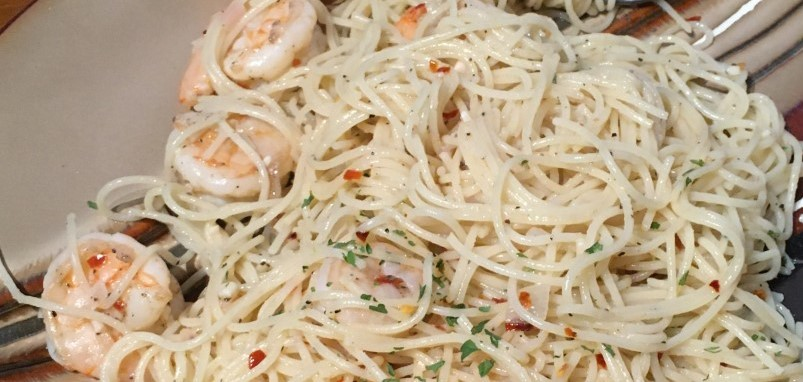
\includegraphics[scale=0.65]{Pasta/Shrimp Scampi/Shrimp Scampi.jpg}
%\end{center}


\end{document}